\chapter{Literature Review}

\section{Related work on ATLASCAR2}

\gls{ad} and \gls{adas} are trendy topics at \gls{lar} in the University of Aveiro. Some research on the ATLASCARs related to \gls{ad} has been made in the past. There are some relevant dissertations done at \gls{lar} that were useful for this project. 

\subsection{Multisensor Calibration and Data Fusion Using LIDAR and Vision} 

This is a master's thesis made by \cite{VieiradaSilva2016}. The work presents an expansion to an existing extrinsic calibration package to vision-based sensors where a ball is used as calibration target. 

The calibration consists in a appearance-based algorithm to detect the ball in the image and a range-based algorithm to detect the ball in the surroundings. 

The calibration package consists in a graphical interface that allows the user to configure the various sensors to be calibrated. The estimated positions between sensors are achieved with sensor data fusion.

\subsection{Visual and Depth Perception Unit for ATLASCAR2} 

This is a master's thesis made by \cite{Correia2017}. It is focused on the installation of an aluminum infrastructure on ATLASCAR 2 to support ranging and vision-based sensors. The sensors setup also include the electrical project in which a power distribution circuit was developed, consisting in the wiring installation and the communication infrastructure. 

In addition, sensor calibration was done using the calibration graphical interface developed by \cite{VieiradaSilva2016}. New sensors were added to the package so that the calibration could be proceeded. To demonstrate the functionalities of the platform setup, a multisensor data merging application was developed representing the free space to navigate around the car.

\subsection{Active Tracking of Dynamic Multivariate Agents} 

This is a PhD Thesis made by \cite{SoaresDeAlmeida2016a}. The thesis is based in the tracking of multiple targets in the fields of advanced safety systems. The focus lies in the prediction of the movement and actions of external agents. Two main targets are studied: vehicles and pedestrians. 

This thesis proposes techniques to improve motion prediction to achieve the development of algorithms capable of target tracking. These algorithms make use of the 3D point clouds of the environment and vision-based sensors. 

\section{Milestones on the History of autonomous driving}

Overall, motorized road transport led to the accidental deaths of around 200,000 US citizens in the 1920s; by far the greatest number of these were pedestrians (\cite{Kroger2016}). The idea of substituting error-prone humans with technology thus practically suggested itself. The first registered experiments for \gls{ad} have been conducted circa the 1920's (\cite{TheMilwaukeeSentinel}) in Milwaukee. A 1926 Chandler was equipped with a transmitting antennae and was radio-controlled by a second car that followed it.

\begin{figure}[htp]
	
	\centering
	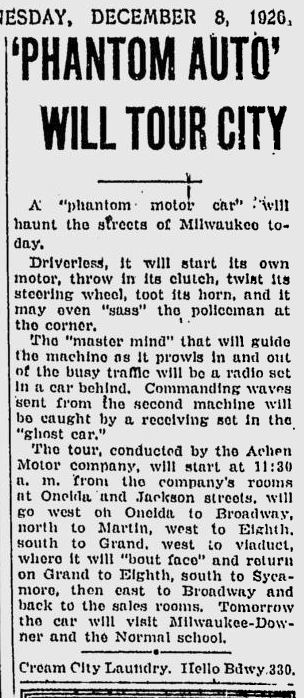
\includegraphics[width=0.25\textwidth]{capstate/imgs/jornal.png}
	
	\caption{The Milwaukee Sentinel - 8 Dez 1926 - 'Phantom Auto' Will Tour City}
	\label{fig:waymo}
	
\end{figure}

In the 1950s promising trials in \gls{ad} took place. General Motors conducted experiments in miniature models along with the electronic manufacturer \gls{rca}. The two companies later developed a full size system that was successfully demonstrated completing a test route of one mile (\cite{Kroger2016}).

In the 1980s, pioneer Ernst Dickmanns designed a vision-guided Mercedes Benz along with the Bundeswehr University Munich engineering team, achieving a speed of 63 km/h on streets with no traffic. In the late 80s, projects with both \gls{lidar} scanners and computer vision were carried out. In 1989 the first experiments with vehicles making use of neural networks were conducted (\cite{Pomerleau1989}).

Various autonomous vehicles competitions have been held. The first long distance competition for driverless cars was the \gls{darpa} Grand Challenge (\cite{DARPA}). The event was open to teams and organizations from around the world. Teams have participated from high schools, universities, businesses and other organizations, bringing a wide variety of technological skills to the race. The challenge offered high value money prizes to the winners. Because the reward was so high, the contest brought various state-of-the-art autonomous vehicles that showcased the solutions implemented in the platforms featuring new ideas that used the most recent technologies.

Since then, many companies and research organizations have been developing various prototype cars. In the past decade, electric motored cars have emerged and new opportunities for \gls{ad} and \gls{adas} research have appeared. 

Waymo, the Google self-driving car project, begun testing driverless cars without someone at the driver position. The Waymo project started in 2009 and it counts more than 5 million miles self-driven. Google has recently partnered with Jaguar and designed self-driving Jaguar I-PACEs (figure \ref{fig:waymo}). Tests on the newest self-driving Waymo's vehicle will be conducted in 2018 (\cite{Waymo}).


\begin{figure}[htp]
	
	\centering
	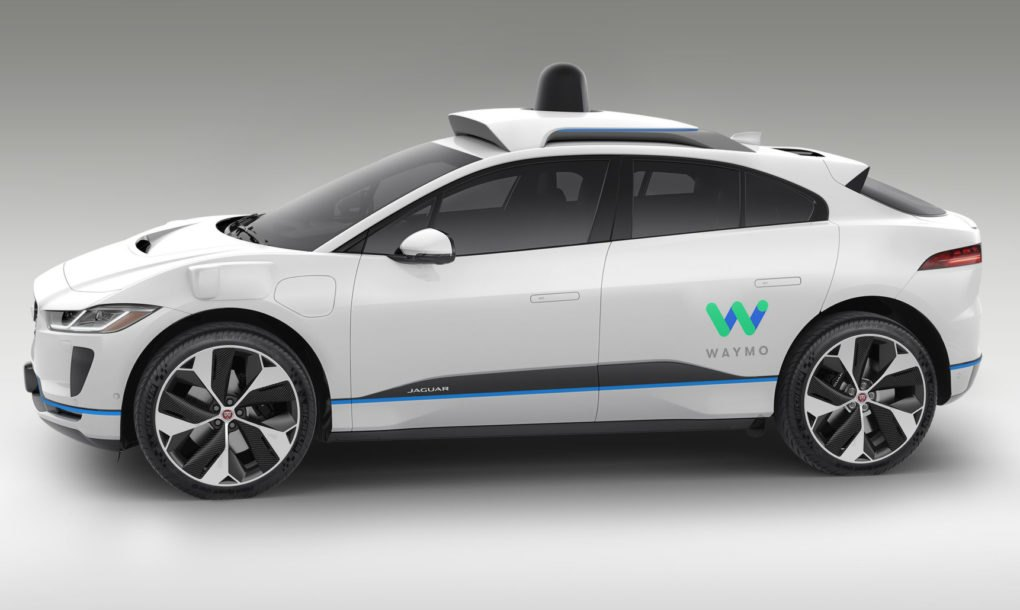
\includegraphics[width=0.9\textwidth]{capstate/imgs/waymo}
	
	\caption{Waymo's Jaguar I-PACE}
	\label{fig:waymo}
	
\end{figure}

Another example of an autonomous vehicle project is the Uber \gls{atc} car based on an hybrid Ford Fusion (figure \ref{fig:uber}). The vehicle is equipped with state of the art \gls{lidar} scanners, and several vision-based sensors and radars.

\begin{figure}[htp]
	
	\centering
	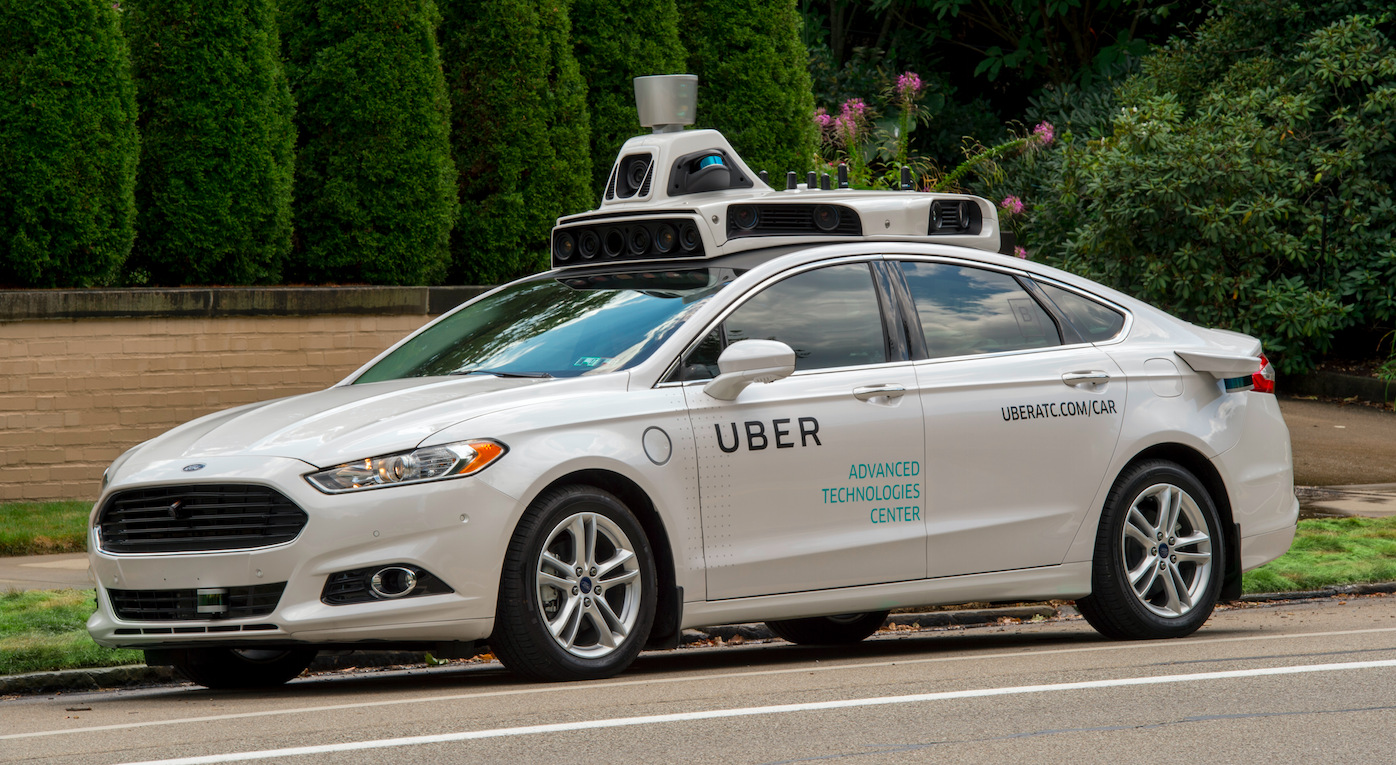
\includegraphics[width=0.9\textwidth]{capstate/imgs/uber}
	
	\caption{Ford Fusion Uber ATC car}
	\label{fig:uber}
	
\end{figure}

Audi released its A8 (figure \ref{fig:audi}) and the company stated that they would be the first manufacturer to use laser scanners in addition to cameras and others sensors in autonomous vehicles. The vehicle was designed to a level 3 autonomous driving: it is capable of self-driving with the expectation that the human driver will respond appropriately to a request to intervene. The Audi AI traffic jam pilot takes over the driving task in slow-moving traffic up to 60 km/h (\cite{AudiMediaCenter}).

\begin{figure}[htp]
	
	\centering
	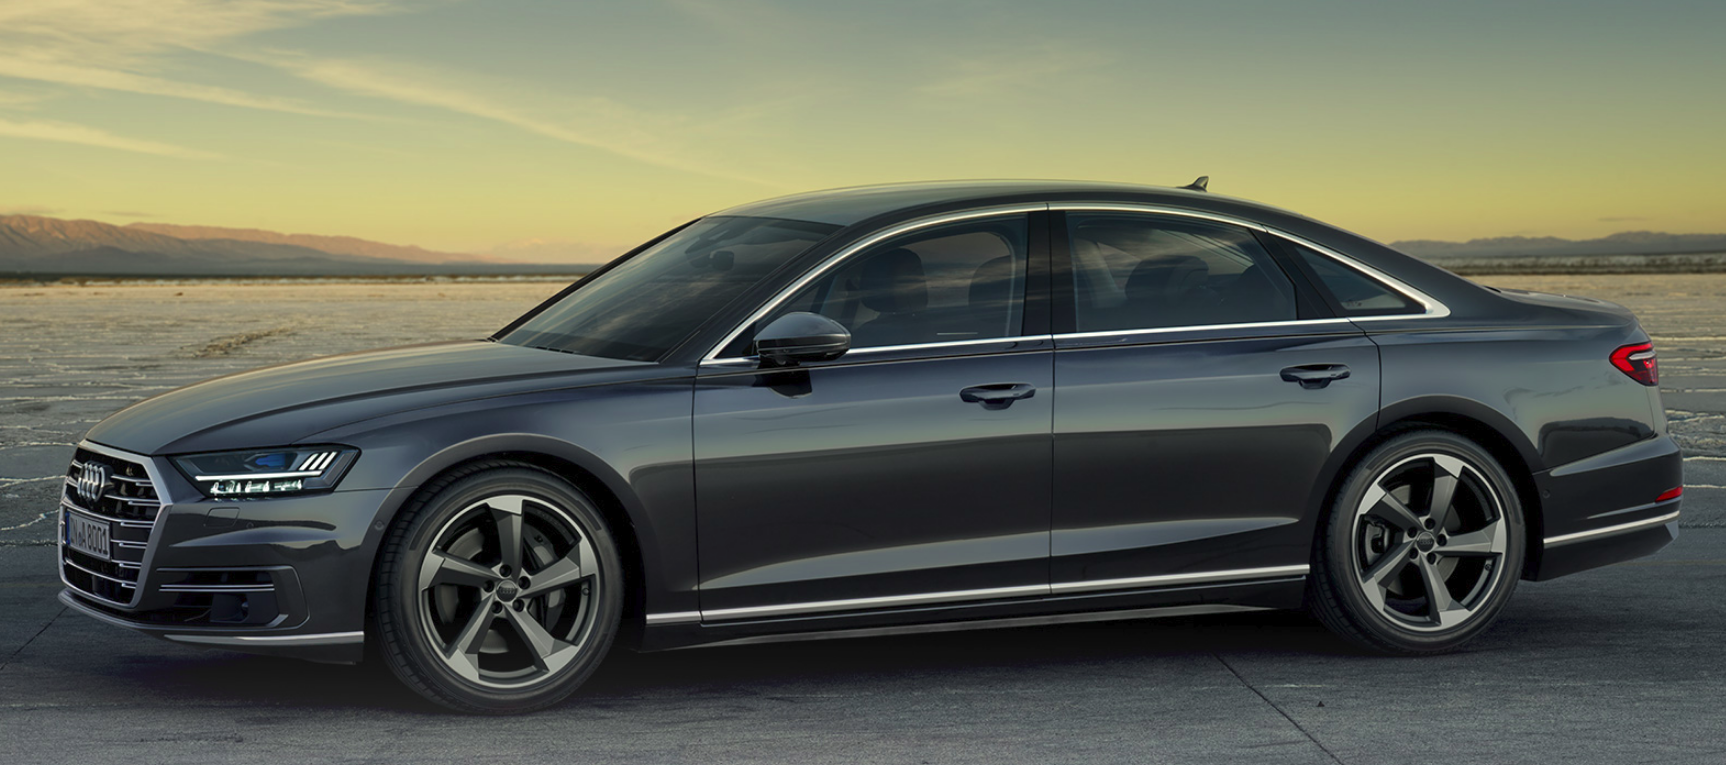
\includegraphics[width=0.9\textwidth]{capstate/imgs/audi}
	
	\caption{The new Audi A8}
	\label{fig:audi}
	
\end{figure}

Like the University of Aveiro, many other universities and research institutes study the \gls{ad} and \gls{adas} paradigms.

Another interesting autonomous vehicle project is the \gls{scot} vehicle (figure \ref{fig:scot}), conducted by the \gls{smart} (\cite{Singapore-MITAllianceforResearchandTechnology}). Like the ATLASCAR 2, \gls{scot} is also a Mitsubishi i-MiEV used to research \gls{adas} and \gls{ad} at \gls{smart} and it is designed for operations on public roads. The \gls{scot} vehicle also relies on \gls{lidar} sensors similar to ATLASCAR 2 (\cite{Teo}). 

\begin{figure}[htp]
	
	\centering
	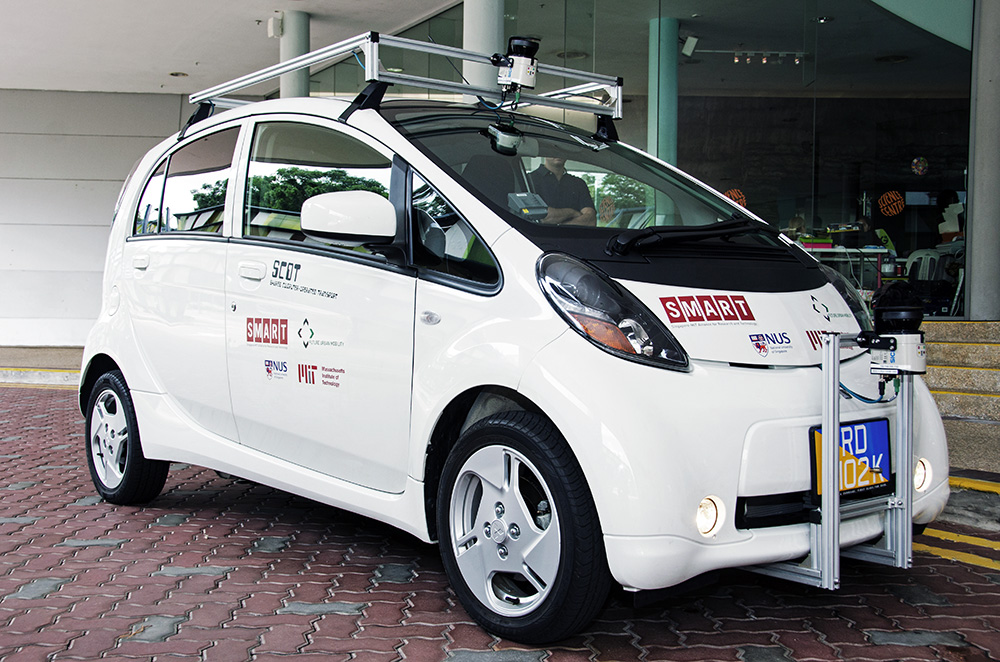
\includegraphics[width=0.9\textwidth]{capstate/imgs/scot}
	
	\caption{SCOT - Shared Computer-Operated Transit vehicle}
	\label{fig:scot}
	
\end{figure}

\begin{figure}[htp]
	
	\centering
	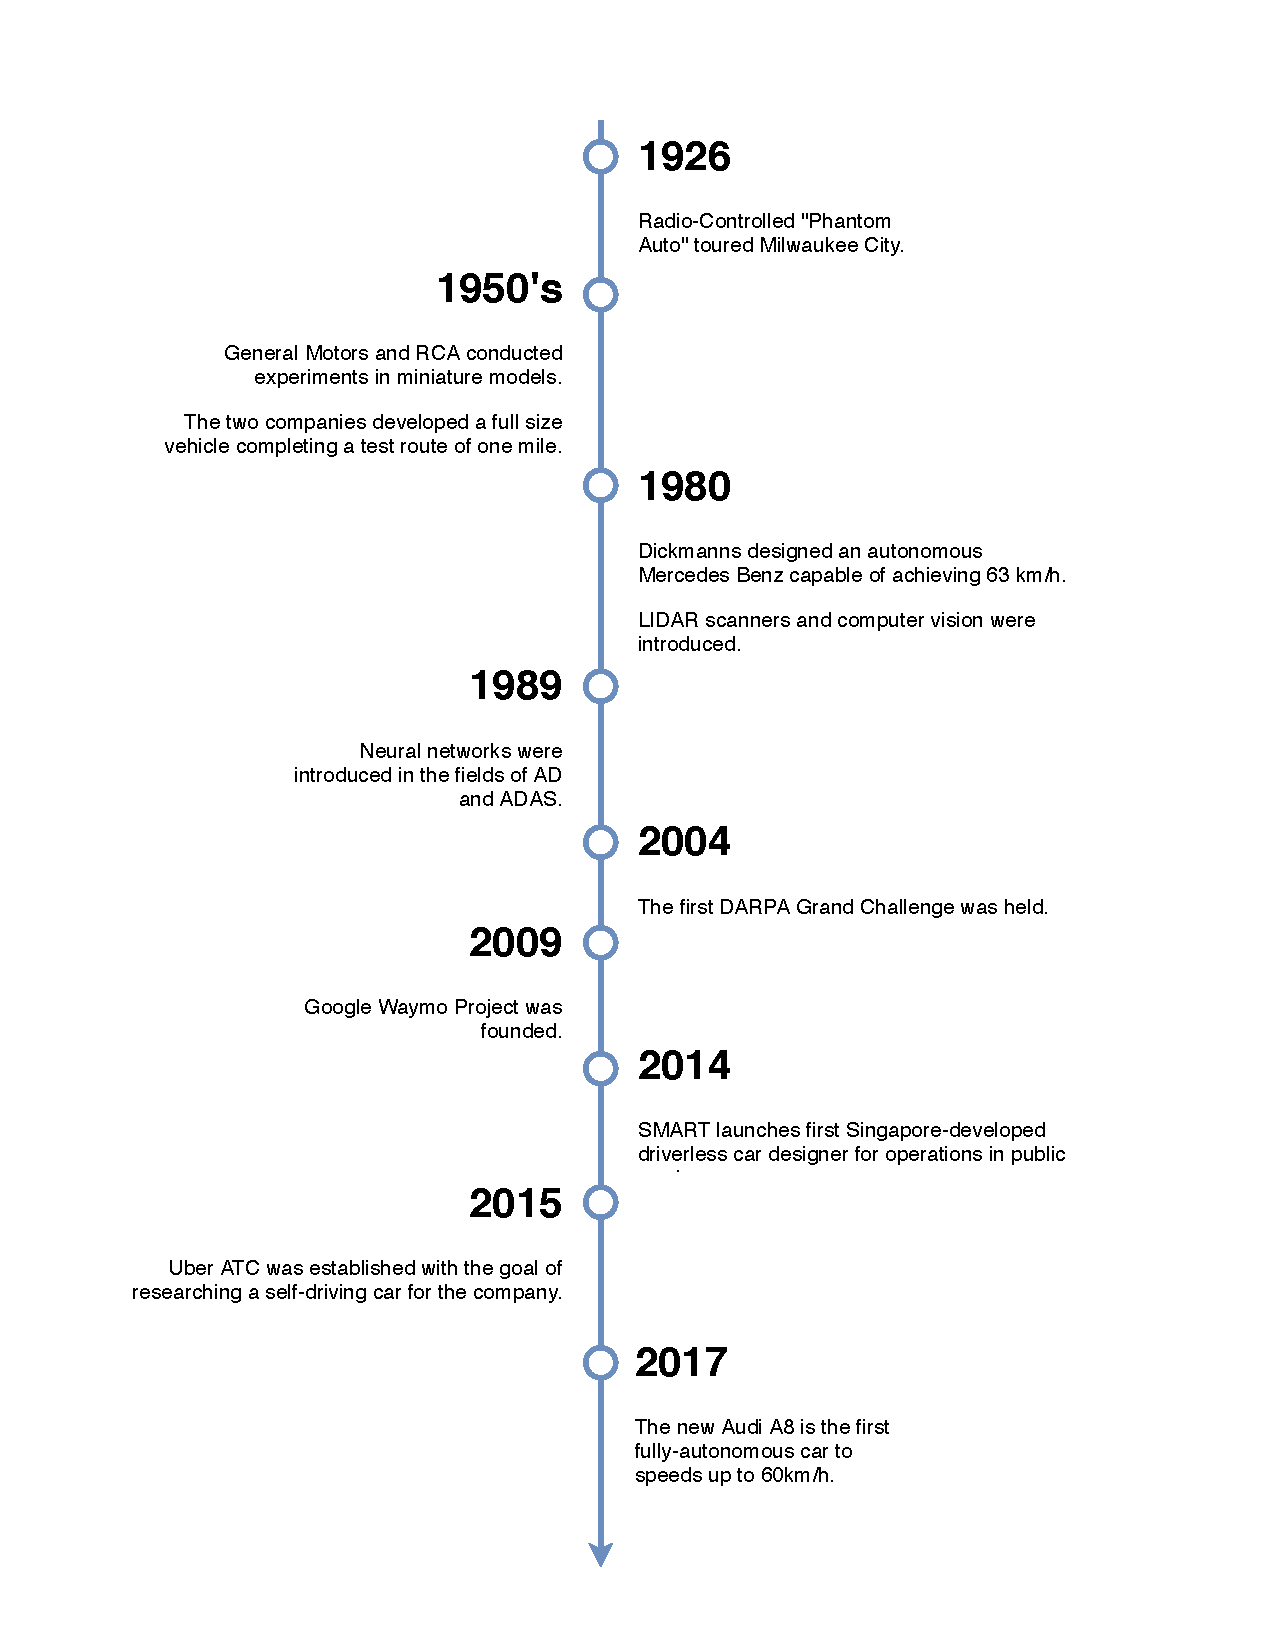
\includegraphics[width=1\textwidth]{capstate/imgs/timeline.pdf}
	
	\caption{Timeline with some milestone of autonomous driving history}
	\label{fig:timeline}
	
\end{figure}

\section{Object Detection and Tracking}
%Fazer um research sobre algoritmos de deteção de objetos%
Computer vision and image processing are often related to algorithms used in object detection. To detect a certain object it is common to look at their geometry and to their color. One of the uses of object detection is tracking its movement. In fixed cameras it is common to use methods like optical flow and background removal. In the fields of \gls{adas} and \gls{ad}, it is assumed that the camera is moving since it belongs to a vehicle, and recently, many car manufacturers already offer automatic pedestrian detection in their latest vehicles. 

To observate traffic the car must be equipped with cameras or laser sensors. To detect a moving object within what is captured in the image and in the laser scans it is needed to implement ways to separate what is the object of interest with the rest. When choosing an object to track it is important to extract its major features in order to identify what object it is. This kind of procedures are related to learning and usually the objects have a classification that connects them to their components.

After gathering information about the select object, the next step is the tracking. All data received from the sensors should be used to maximize precision and accuracy of the objects position. For the camera there is a 2D position relatively to the coordinates of the object in the image view. In the other hand, the laser sensors can create tridimensional pointclouds, so the target's position can be anywhere in space. 

With images it is common to use the template matching strategy to track objects within the field of view. The object features are gathered and can be used to find where the object is in the next frame. In range based sensors the objects are detected by separating the nearest points of the position of interest from the farthest. The points are tracked and based on their direction and velocity it can be calculated an estimate location when the tracking is lost.

\section{Labelling Datasets}
Tracking of objects in images is done frequently using bounding boxes around the target. These boxes are often linked to a class in which the object in the template represents. Image labelling is the act of relating the object to this class, or more specifically, the label. Some image labelling datasets already exist and in this section it will be presented a few used in the research of this dissertation.

\subsection{KITTI Dataset}
One of them and probably the most well-known in the fields of \gls{ad} is the \gls{kitti} dataset (\cite{KarlsruheInstituteofTechnology}). The \gls{kitti} Dataset was captured with a Volkswagen station wagon (figure \ref{fig:kitticar}) for use in mobile robotics and \gls{ad} research. The \gls{kitti} benchmark suite is born in 2012 at Karlsruhe Institute of Technology by the need to have a dataset to classify objects on the streets. 

This project has grown by increasingly adding more results with more sensors. The \gls{kitti} benchmark started with the stereo, flow and odometry benchmarks and today it includes standards for object tracking and more. 

\begin{figure}[htp]
	
	\centering
	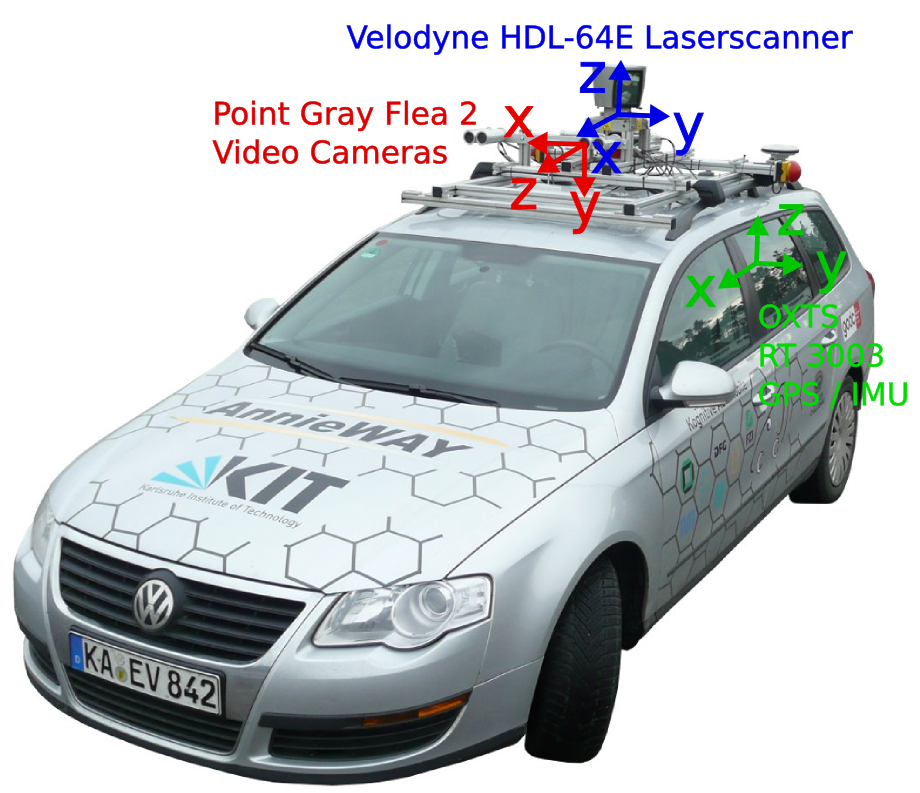
\includegraphics[width=0.7\textwidth]{capstate/imgs/kitticar}
	
	\caption{Volkswagen Station Wagon used in the KITTI Dataset}
	\label{fig:kitticar}
	
\end{figure}

Just like ATLASCAR 2, the car used in the \gls{kitti} dataset is equipped with \gls{lidar} sensors and Point Grey Video Cameras. The dataset is used for automatic recognition and tracking of vehicles and pedestrians. 

It consists in image sequences (see figure \ref{fig:kittiresult}) and a text file in which, for each frame the various objects in the field of view are depicted with and identification number, a label, and coordinates about their position regarding the car and in the image ( \cite{Geiger}). 

The development kit used for the KITTI database contains C++ and MATLAB code to read the sensor data and write dataset results. The data development kit used is provided on the KITTI Website (\cite{KarlsruheInstituteofTechnology}). It contains MATLAB demonstration code with C++ wrappers. 

The data is manipulated to be inserted into MATLAB structures and arrays. The demonstration shows how 3D boxes can be read from the dataset files and projected into the image plane of the cameras (see figure \ref{fig:kittidk}). The KITTI database also uses the \gls{pcl} to process and gather the pointclouds obtained from the LIDAR sensors.

\begin{figure}[htp]
	
	\centering
	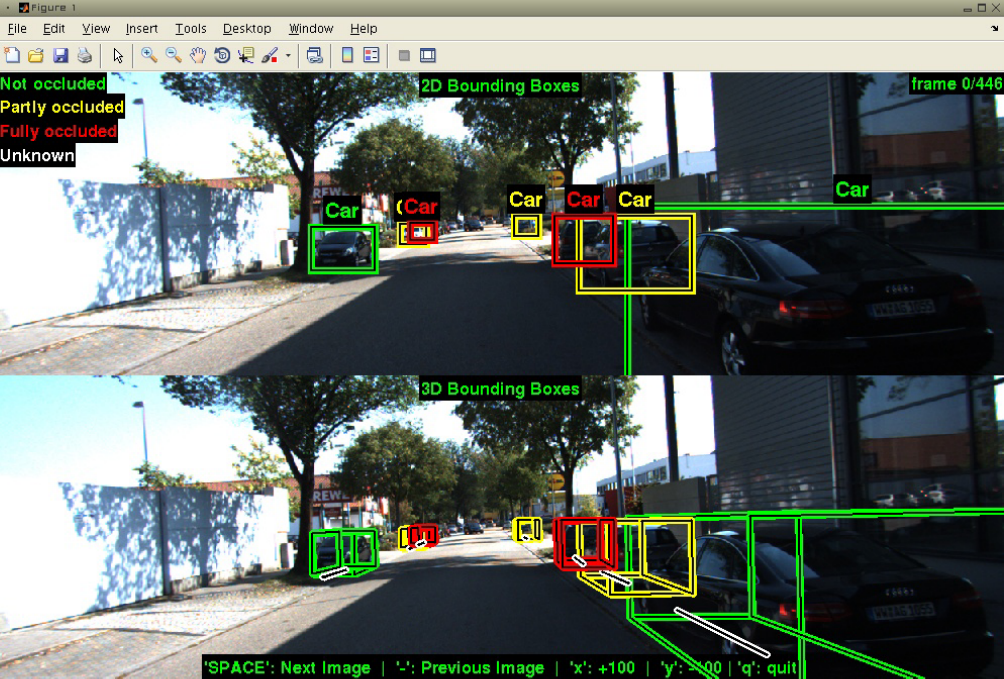
\includegraphics[width=0.85\textwidth]{capstate/imgs/kittidk.png}
	
	\caption{KITTI development kit showing 2D and 3D bounding boxes around several cars}
	\label{fig:kittidk}
	
\end{figure}

\begin{figure}
\begin{center}
	\begin{lstlisting}[caption={KITTI dataset file snippet.}, language=c++, label={lst: pop_grid}]
	...
	3 1 Cyclist 0 0 -1.931469 759.786603 146.098339 954.280160 374.000000 1.739063 0.824591 1.785241 1.821119 1.569936 5.783265 -1.642450
	3 2 Pedestrian 0 0 -2.547728 1154.836779 148.360923 1241.000000 321.627088 1.714062 0.767881 0.972283 6.463579 1.474131 7.560739 -1.860031
	4 -1 DontCare -1 -1 -10.000000 252.530000 168.660000 284.460000 202.850000 -1000.000000 -1000.000000 -1000.000000 -10.000000 -1.000000 -1.000000 -1.000000
	4 0 Van 0 0 -1.808333 290.287584 146.641981 444.387179 269.473545 2.000000 1.823255 4.433886 -4.934786 1.601945 14.098646 -2.139796
	4 1 Cyclist 0 0 -1.929519 767.158958 140.942948 961.992360 374.000000 1.739063 0.824591 1.785241 1.881359 1.534695 5.785600 -1.631447
	4 2 Pedestrian 1 0 -2.557045 1180.675035 151.025283 1241.000000 325.015204 1.714062 0.767881 0.972283 6.516488 1.497786 7.267796 -1.846627
	...	\end{lstlisting}
\end{center}
\end{figure}

Listing \ref{lst: pop_grid} shows an example snippet in which there are two lines of what the \gls{kitti} dataset looks like. Each line starts with the frame ID and the ID of the object being tracked. Then it is added a label to classify this object. There are also flags to indicate if the object is either truncated or occluded in the image sequence. 

The following numbers consist in the alpha (observation angle of object), the left, top, right and bottom of the 2D bounding box, the height, width and length of the 3D bounding box and its XYZ coordinates. The last number consists in the 3D rotation angle in the Y axis (\cite{Team}).

\begin{center}
	\begin{lstlisting}[caption={KITTI dataset file snippet legend.}, label={lst: kitti_legend}]
	frame_id object_id label truncated occluded alpha left top right bottom height width length x y z rotation_y	\end{lstlisting}
\end{center}

The legend of the KITTI datasets is in listing \ref{lst: kitti_legend} but it is not included in the dataset files. Analyzing the snippet, it is possible to locate a a cyclist and a pedestrian in frame 3 and the same cyclist and pedestrian (because they have the same object\_id) in the next frame with also a van. The \texttt{DontCare} label is often shown representing an object detected that is not related to the scope of the \gls{kitti} dataset. Other information indicate where these objects are found relatively to the car.

\begin{figure}[htp]
	
	\centering
	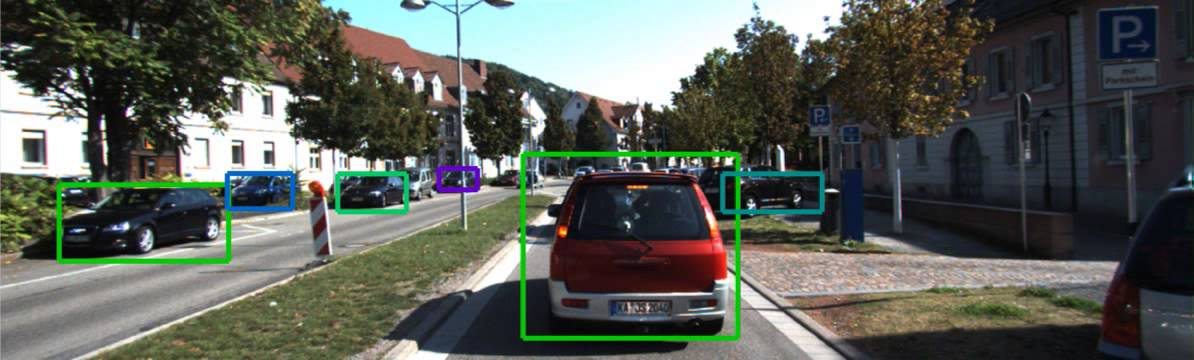
\includegraphics[width=0.99\textwidth]{capstate/imgs/kittiresult}
	
	\caption{Sequence example of tracking by detection using the \gls{kitti} dataset}
	\label{fig:kittiresult}
	
\end{figure}
	
\subsection{HumanEva II Dataset}
The HumanEva II Dataset from the \gls{mpii} was also an interesting dataset. Although it is used for pedestrian detection only, it was important to have a comparator with the \gls{kitti} dataset, specially regarding its structure. 

This dataset appears with the need to represent information about detection and tracking of humans and their poses captured by a single image camera. The HumanEva dataset development kit includes several MATLAB modules, each one implementing a feature. Some modules refer to the body pose, others to image stream processing, writing the dataset results, and so on. Each script implements a chunk of the system that gathers the data and shapes it into MATLAB structures to be processed and to create the dataset.

The HumanEva dataset has information about the bounding boxes position used to track and detect pedestrian limb poses. This information is useful to know which direction the person is facing from the 3D skeleton derived from the pose. The data structure in the dataset is similar to a XML file. For each frame in the image sequences there are several bounding boxes with the respective coordinates (\cite{Sigal}).

\begin{figure}
\lstinputlisting[label={lst:humaneva_snip}, caption={HumanEva dataset file snippet.},language=xml]{capstate/files/humaneva_snip.xml}
\end{figure}

\begin{figure}[htp]
	
	\centering
	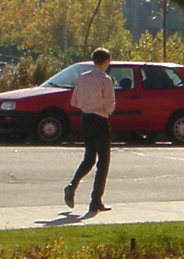
\includegraphics[width=0.5\textwidth]{capstate/imgs/00050.png}
	
	\caption{Example image of the HumanEva dataset that generated the snippet in listing \ref{lst:humaneva_snip} }
	\label{fig:00050}
	
\end{figure}

By looking at listing \ref{lst:humaneva_snip}, in this dataset snippet is easy to identify the interest points in the given frame. The files are a set of annotations called $annotationList$ in which a path to the image corresponding to the frame is given. For each image there are several bounding boxes with coordinates $(x1,y1,x2,y2)$, a score, silhouette, articulation and viewpoint id.

\subsection{Other relevant datasets}
Other datasets included in the research for this dissertation are found in \gls{ethz} and in \gls{epfl} projects. 
\subsubsection{ETHZ dataset}
\gls{ethz} conducted studies for detection and tracking of people on the street. Just like the previous datasets, the development is based in MATLAB scripts and the data is gathered and stored in MATLAB structures. The dataset is simple: for each frame there are several bounding boxes in the image.
\begin{figure}
\begin{center}
	\begin{lstlisting}[label={lst:ETHZ}, caption={ETHZ dataset dataset file snippet.},language=c++]
	...
	"left/image_00000015_0.png": (222, 177, 268, 312), (373, 105, 463, 393), (458, 220, 487, 285), (310, 225, 327, 265), (335, 228, 352, 264), (267, 228, 281, 261);
	"left/image_00000016_0.png": (220, 172, 266, 313), (378, 407, 476, 102), (462, 219, 486, 285), (312, 223, 327, 264), (337, 226, 352, 262), (267, 231, 279, 260);
	"left/image_00000017_0.png": (219, 173, 267, 316), (394, 94, 489, 423), (313, 222, 330, 262), (338, 227, 354, 262), (267, 228, 279, 260);
	...	\end{lstlisting}
\end{center}
\end{figure}

\begin{figure}[htp]
	
	\centering
	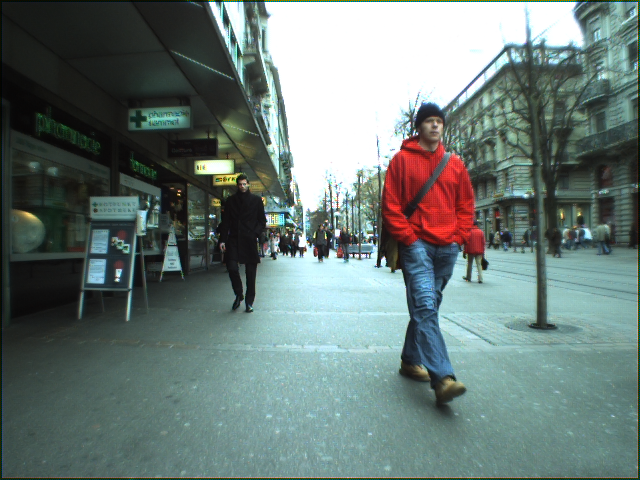
\includegraphics[width=0.7\textwidth]{capstate/imgs/image_00000016_0.png}
	
	\caption{One of the images of the \gls{ethz} dataset that generated part of the snippet in listing \ref{lst:ETHZ} }
	\label{fig:ETHZ}
	
\end{figure}

This dataset is focused just in the detection and tracking of pedestrians in the image (\cite{ETHZEidgenossischeTechnischeHochschuleZurich}). In listing \ref{lst:ETHZ} each line is composed with a string defining a path to the image representing the actual frame, followed by tuples of four elements $(x1,y1,x2,y2)$ representing the bounding boxes where pedestrians are found in the respective frame. 

\subsubsection{EPFL dataset}
The \gls{epfl} designed a dataset for multiple people in a camera environment, independent of the scenario. This dataset used various synced video cameras filming the same area in different angles. The data from the cameras is captured and processed with MATLAB scripts. This dataset also features some algorithms in C++.

\begin{figure}
\begin{center}
	\begin{lstlisting}[label={lst:basket}, caption={ETHZ dataset file snippet.},language=c++]
									...
									1 80 45 99 98 9363 0 0 1 "PERSON"
									1 80 45 99 98 9364 0 0 0 "PERSON"
									1 77 45 96 98 9365 0 0 1 "PERSON"
									1 74 45 93 98 9366 0 0 1 "PERSON"
									1 71 46 90 99 9367 0 0 0 "PERSON"
									2 81 45 110 126 0 0 0 0 "PERSON"
									2 80 45 109 126 1 0 0 1 "PERSON"
									2 80 45 109 126 2 0 0 1 "PERSON"
									2 80 45 109 126 3 0 0 1 "PERSON"
									2 80 45 109 126 4 0 0 1 "PERSON"
									...	\end{lstlisting}
\end{center}
\end{figure}

\begin{figure}[htp]
	
	\centering
	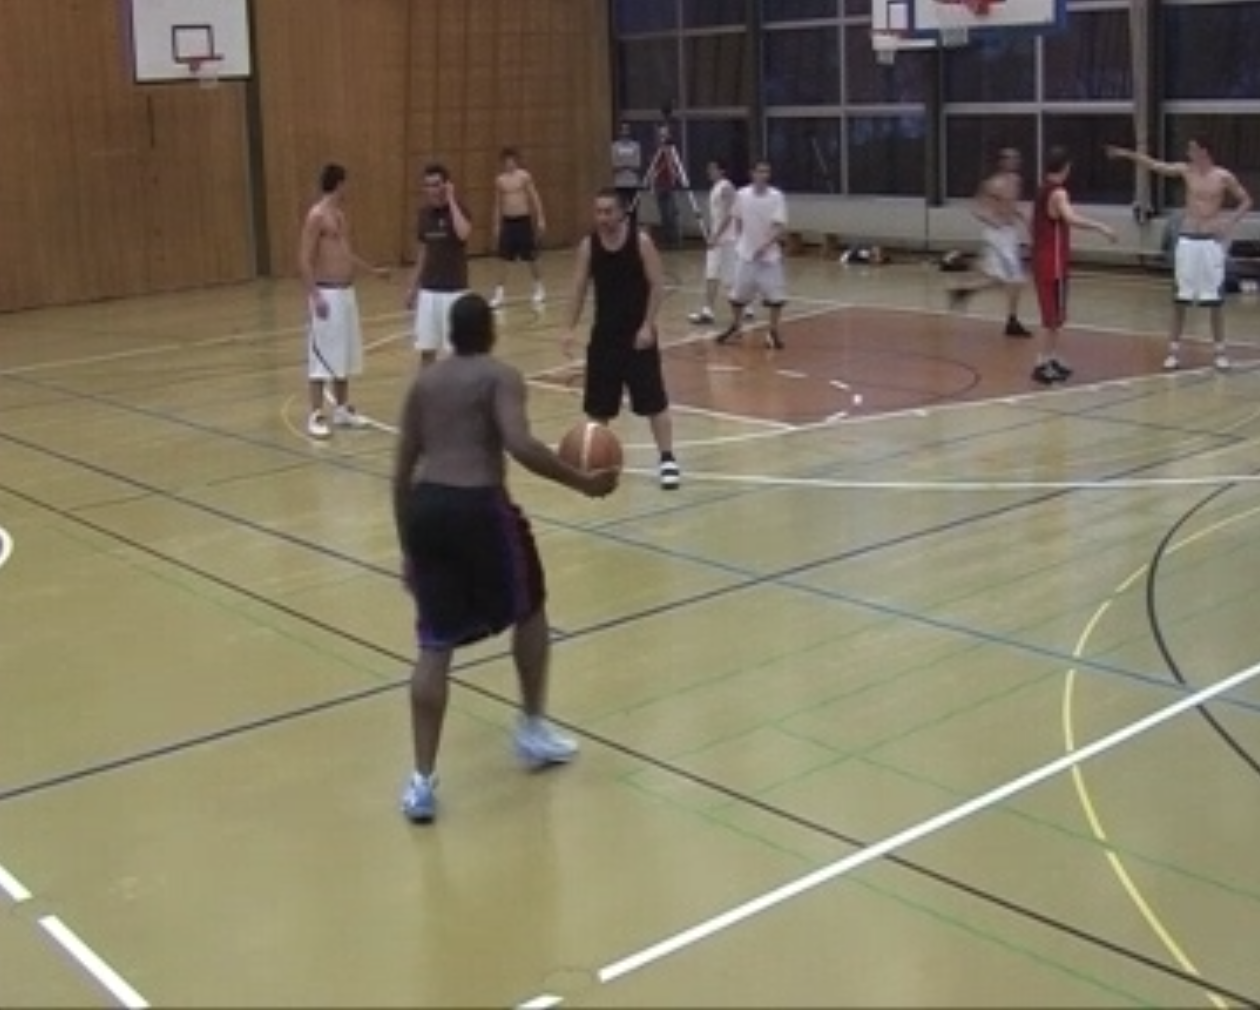
\includegraphics[width=0.7\textwidth]{capstate/imgs/basket.png}
	
	\caption{One of the images of the \gls{epfl} dataset that generated part of the snippet in listing \ref{lst:basket} }
	\label{fig:basketimg}
	
\end{figure}


In listing \ref{lst:basket} there is a snippet of the dataset. The dataset includes, for each frame, various objects identified with a number, a label, bounding box coordinates, and flags to point out if the person is occluded, lost, or if the detection was automatically interpolated from the other camera's information ( \cite{EPFLEcolepolytechniquefederaledeLausanne}). The particularity of the structure of this dataset is that, for each object, it is tracked in the image sequences individually, and only then another object is tracked and labeled. In listing \ref{lst:basket_leg} a legend of this dataset can be found.

\begin{figure}[htp]

\begin{center}
	\begin{lstlisting}[label={lst:basket_leg}, caption={EPFL dataset legend.}]
	track_id. All rows with the same ID belong to the same path.
	xmin. The top left x-coordinate of the bounding box.
	ymin. The top left y-coordinate of the bounding box.
	xmax. The bottom right x-coordinate of the bounding box.
	ymax. The bottom right y-coordinate of the bounding box.
	frame_number. The frame that this annotation represents.
	lost. If 1, the annotation is outside of the view screen.
	occluded. If 1, the annotation is occluded.
	generated. If 1, the annotation was automatically interpolated.
	label. (human, car/vehicle, bicycle...)	\end{lstlisting}
\end{center}

\end{figure}
 



